% !TeX root = ../../../main.tex

The fraction of the proton momentum carried by charm quarks
is given by
\begin{equation}
\label{eq:ic/charm_momentum_fraction}
\left[ c\right] = \int_0^1dx\, x c^+(x,Q^2) \, .
\end{equation}
Model predictions, as mentioned, are typically provided up to an
overall normalization, which in turn determines the charm momentum fraction.
%
Consequently, the momentum fraction is often cited as a characteristic
parameter of intrinsic charm.
%
It should however be borne in mind that,
even in the absence of intrinsic charm, this charm momentum fraction is nonzero due
to the perturbative contribution.

In Table~\ref{tab:ic/momfrac_lowQ} we indicate
the values of the charm momentum fraction
 in the 3\fns for our default charm
  determination and in the 4\fns  (at $Q=1.65$ GeV) both for the
  default result and for perturbative charm \pdf (see SI Sect.~\ref{sec:ic/consistency}).
%
We provide results for  three different values of the charm mass $m_c$ and
indicate separately the \pdf and the MHO uncertainties.
%
The 3\fns result is scale-independent, it corresponds to the
momentum fraction carried by intrinsic charm, and it vanishes identically
by assumption in the perturbative charm case.
%
The 4\fns result corresponds to
the scale-dependent momentum fraction that combines the intrinsic and
perturbative contribution, while of course it contains only the
perturbative contribution in the case of perturbative charm.
%
As
discussed in SI Sect.~\ref{sec:ic/consistency}, the large uncertainty
associated to higher order corrections to the matching conditions
affects the 3\fns result (intrinsic charm) in the default case, in
which the charm \pdf is determined from data in the 4\fns scheme, while
it affects the 4\fns result for perturbative charm, that is determined
assuming the vanishing of the 3\fns result.

 For our default determination, the charm
momentum fraction in the 4\fns at low scale
differs from zero at the $3\sigma$
level.
%
However, it is not possible to tell whether this is of
perturbative or intrinsic origin, because, due to  the large MHOU in
the matching condition, the intrinsic (3\fns) charm momentum fraction
is compatible with zero. This large uncertainty is entirely due to the
small $x\lsim 0.2$ region, see see
Fig.~\ref{fig:ic/charm_content_3fns}~(right).
%
Accordingly, for perturbative charm the
low-scale 4\fns
momentum fraction is compatible with zero.
%
Consistently with the results of SI Sect.~\ref{sec:ic/charm_stability_4fns},
the 4\fns result is essentially independent of the value of the charm
mass, but it becomes strongly dependent on it if one assumes
perturbative charm.

%%%%%%%%%%%%%%%%%%%%%%%%%%%%%%%%%%%%%%%%%%%%%%%%%%%%%%%%%%%%%%%%%%%%%%%%%%%%%%%
\begin{table}[t]
  \footnotesize
  \centering
    \renewcommand{\arraystretch}{1.30}
\begin{tabularx}{\textwidth}{C{2.0cm}C{2.3cm}C{2.2cm}C{2.2cm}C{5.6cm}}
  \toprule
  Scheme  & $Q$ & Charm \pdf & $m_c$  &  $\left[ c\right]~\left(\%\right)$ \\
  \midrule
  \midrule
 3\fns  & --  &default  &  1.51 GeV  &   $ 0.62\pm0.28_\textrm{ pdf}\pm 0.54_\textrm{ mhou} $ \\
 3\fns  & --  &default  &  1.38 GeV  &   $ 0.47\pm0.27_\textrm{ pdf}\pm 0.62_\textrm{ mhou} $ \\
 3\fns  & --  &default  &  1.64 GeV  &    $ 0.77\pm0.28_\textrm{
  pdf}\pm 0.48_\textrm{ mhou} $ \\
  \midrule

 4\fns  & 1.65 GeV  & default  &  1.51 GeV  &   $0.87 \pm 0.23_\textrm{ pdf}$  \\
 4\fns  & 1.65 GeV  & default &  1.38 GeV  &   $0.94 \pm 0.22_\textrm{ pdf}$  \\
 4\fns  & 1.65 GeV  & default   &  1.64 GeV  &  $0.84 \pm 0.24_\textrm{ pdf}$  \\
  \midrule
 \midrule
 4\fns  & 1.65 GeV   & perturbative  &  1.51 GeV  &   $0.346\pm 0.005_\textrm{ pdf}\pm 0.44_\textrm{ mhou}$ \\
 4\fns  & 1.65 GeV   & perturbative  &  1.38 GeV  &    $0.536\pm 0.006_\textrm{ pdf}\pm 0.49_\textrm{ mhou}$ \\
 4\fns  & 1.65 GeV   & perturbative  &  1.64 GeV  &    $0.172\pm 0.003_\textrm{ pdf}\pm 0.41_\textrm{ mhou}$ \\
\bottomrule
\end{tabularx}
\vspace{0.3cm}
\caption{\label{tab:ic/momfrac_lowQ}
  The charm momentum fraction, Eq.~(\ref{eq:ic/charm_momentum_fraction}).
  %
  We show  results both in the 3\fns and the 4\fns (at $Q=1.65$ GeV)
  for our default charm, and also in the 4\fns for perturbative charm.
  %
We provide results for  three different values of the charm mass $m_c$ and
indicate separately the \pdf and the MHO uncertainties.
}
\end{table}
%%%%%%%%%%%%%%%%%%%%%%%%%%%%%%%%%%%%%%%%%%%%%%%%%%%%%%%%%%%%%%%%%%%%%%%%%%%%%%%

%%%%%%%%%%%%%%%%%%%%%%%%%%%%%%%%%%%%%%%%%%%%%%%%%%%%%%%%%%%%%%%%%%%
\begin{figure}[h]
  \begin{center}
     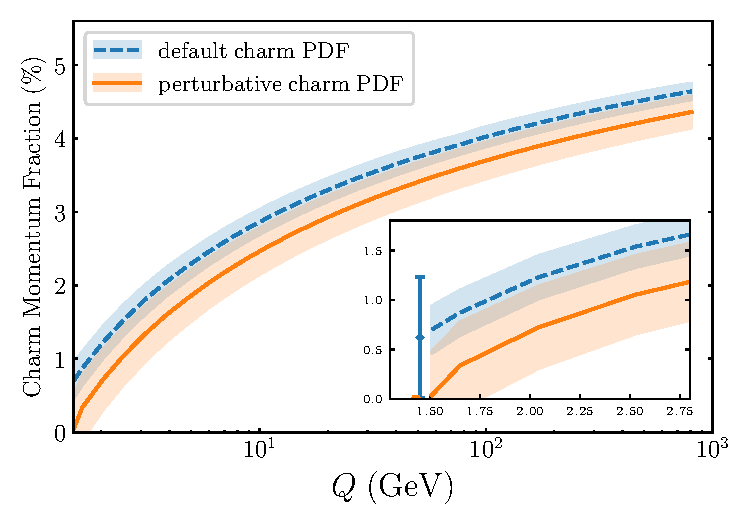
\includegraphics[width=0.60\linewidth]{ch-ic/charm_momfrac_qdep.pdf}
    \caption{\small 
      The 4\fns charm momentum fraction in NNPDF4.0 as a function of scale $Q$,
      both for the default and perturbative charm cases,
      for a charm mass value of $m_c=1.51$ GeV.
      %
     The inset zooms on the low-$Q$ region and includes the 3\fns
     (default) result
     from Table~\ref{tab:ic/momfrac_lowQ}. 
     %
     Note that the uncertainty includes the MHOU for the 3\fns default
     and 4\fns perturbative charm cases, while it is the \pdf
     uncertainty for the 4\fns default charm case.
  \label{fig:ic/comparison_IC_models} }
\end{center}
\end{figure}
%%%%%%%%%%%%%%%%%%%%%%%%%%%%%%%%%%%%%%%%%%%%%%%%%%%%%%%%%%%%%%%%%%%%%%

The 4\fns charm momentum fraction is plotted as a function of scale
in Fig.~\ref{fig:ic/comparison_IC_models}, both in the default case and
for perturbative charm, with the 3\fns values and the detail of the low-$Q$ 
4\fns results shown in an inset.
%
The dependence on the value of the charm mass
is shown in Fig.~\ref{fig:ic/charm_momfrac_qdep_mc}.
The large MHOUs on the 3\fns result, and on the 
4\fns result in the case of perturbative charm, are apparent.
The stability of the default result upon variation of  the value of
$m_c$, and the strong dependence of the perturbative charm result on
$m_c$, are  also clear.
Both the large MHOU uncertainty, and the strong dependence on
the value of $m_c$
for perturbative charm are seen to persist up to large scales.


%%%%%%%%%%%%%%%%%%%%%%%%%%%%%%%%%%%%%%%%%%%%%%%%%%%%%%%%%%%%%%%%%%%
\begin{figure}[t]
  \begin{center}
    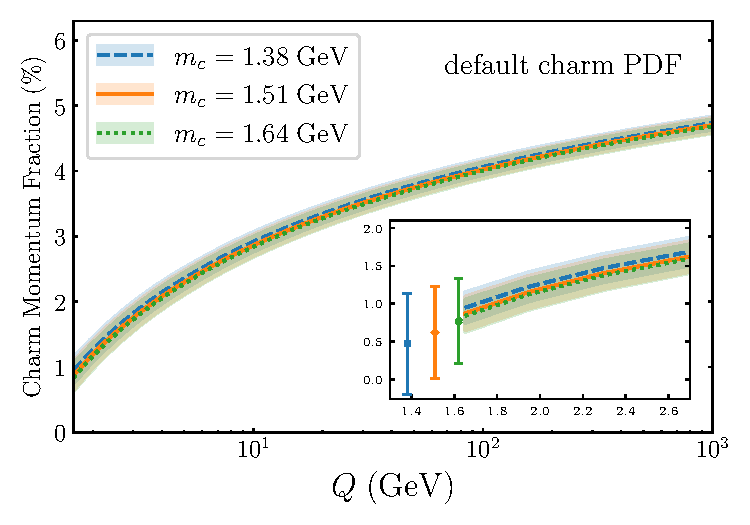
\includegraphics[width=0.49\linewidth]{ch-ic/charm_momfrac_qdep_mc.pdf}
    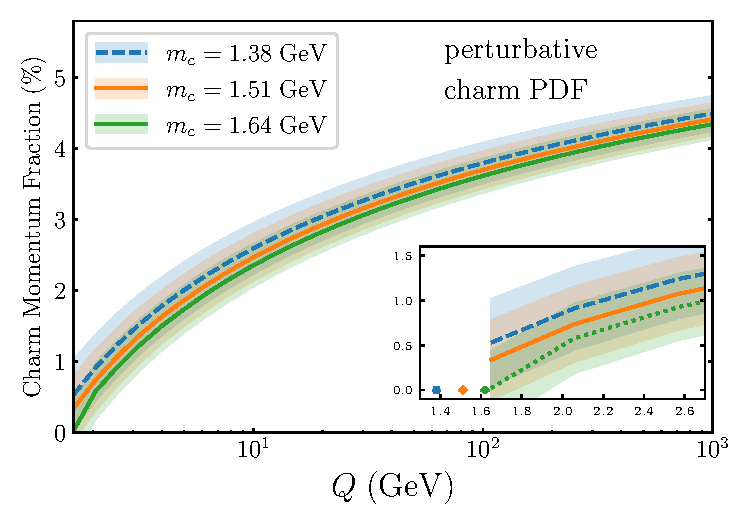
\includegraphics[width=0.49\linewidth]{ch-ic/charm_momfrac_qdep_mc_pert.pdf}
    \caption{\small
    Same as Fig.~\ref{fig:ic/comparison_IC_models} for different values
    of the charm mass. Note that the 3\fns momentum fraction for
     perturbative charm vanishes identically by assumption.
   \label{fig:ic/charm_momfrac_qdep_mc} }
\end{center}
\end{figure}
%%%%%%%%%%%%%%%%%%%%%%%%%%%%%%%%%%%%%%%%%%%%%%%%%%%%%%%%%%%%%%%%%

It is interesting to understand in detail the impact of the MHOU on
the momentum fraction carried by intrinsic charm. To this purpose, we
have computed  the truncated momentum integral, i.e.\ 
  Eq.~(\ref{eq:ic/charm_momentum_fraction}) but only integrated down to
  some  lower
  integration limit $x_\textrm{ min}$:
  \begin{equation}
\label{eq:ic/charm_momentum_fraction_truncated}
\left[ c\right]_\textrm{ tr}(x_\textrm{ min}) \equiv \int_{x_\textrm{ min}}^1dx\, x c^+(x,Q^2) \, .
\end{equation}
Note than in the 3\fns   $x
c^+(x)$ does not depend on scale, so  this becomes
a scale-independent quantity.
%
The result for our default intrinsic charm determination is displayed
in Fig.~\ref{fig:ic/charm_momfrac_xmin_dep}, as a function of
of the lower integration limit $x_\textrm{ min}$.
%
It is clear that for $x_\textrm{ min} \gtrsim 0.2$ the truncated momentum
fraction  differs significantly from zero, thereby providing evidence
for intrinsic charm with similar statistical  significance as the
local pull shown in Fig.~\ref{fig:ic/Zc} bottom left.
%
For $x \lsim 0.2$
this  significance is then washed out
by the large MHOUs.

Hence, while the total momentum fraction has been traditionally adopted
as a measure of intrinsic charm, 
our analysis shows that, once MHOUs are accounted for, the information
provided by the total momentum fraction is limited, at least with
current data and theory.



%%%%%%%%%%%%%%%%%%%%%%%%%%%%%%%%%%%%%%%%%%%%%%%%%%%%%%%%%%%%%%%%%%%
\begin{figure}[h!]
  \begin{center}
    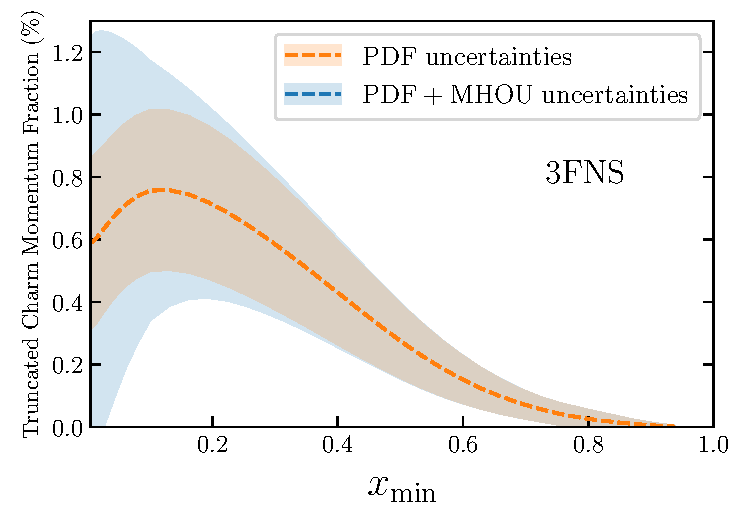
\includegraphics[width=0.65\linewidth]{ch-ic/charm_momfrac_xmin_dep_3fns.pdf}
    \caption{\small The value of the truncated charm momentum integral,
      Eq.~(\ref{eq:ic/charm_momentum_fraction_truncated}), as a function
      of the lower integration limit $x_\textrm{ min}$
      for our baseline determination of the 3\fns intrinsic charm \pdf.
      %
      We display separately the \pdf and the total (\pdf+MHOU) uncertainties.
  \label{fig:ic/charm_momfrac_xmin_dep} }
\end{center}
\end{figure}
%%%%%%%%%%%%%%%%%%%%%%%%%%%%%%%%%%%%%%%%%%%%%%%%%%%%%%%%%%%%%%%%%%%%%%
